\chapter{Spendley's et al. method}

\section{Analysis}

The simplex algorithms are based on the iterative update of 
a \emph{simplex} made of $n+1$ points $S={x_i}_{i=1,n+1}$. Each point 
in the simplex is called a \emph{vertex} and is associated with 
a function value $f_i=f(x_i), i=1,n+1$.

The vertices are sorted by increasing function values so that the 
\emph{best} vertex has index 1 and the \emph{worst} vertex 
has index $n+1$

\begin{eqnarray}
\label{sorted-vertices-fv}
f_1 \leq f_2 \leq \ldots \leq f_n \leq f_{n+1}.
\end{eqnarray}

The \emph{next-to-worst} vertex with index $n$ has a 
special role in simplex algorithms.

The centroid of the simplex is the center of the vertices
where the vertex with index $j=1,n+1$ has been 
excluded 

\begin{eqnarray}
\label{centroid-generalized}
\overline{x} (j) = \frac{1}{n} \sum_{i=1,n+1, i\neq j}x_i
\end{eqnarray}

The first move of the algorithm is based on the centroid 
where the worst vertex with index $j=n+1$ has been excluded 

\begin{eqnarray}
\label{centroid-worst}
\overline{x} (n+1) = \frac{1}{n} \sum_{i=1,n}x_i
\end{eqnarray}

The algorithm attemps to replace one vertex 
$x_j$ by a new point $x(\mu,j)$ between the centroid 
$\overline{x}$ and the vertex $x_j$ and defined by 
\begin{eqnarray}
\label{interpolate-generalized}
x(\mu,j) = (1+\mu)\overline{x}(j) - \mu x_j
\end{eqnarray}

The Spendley et al. \cite{Spendley1962} algorithm makes use
of one coefficient, the reflection $\rho>0$. The standard
value of this coefficient is $\rho=1$.

The first move of the algorithm is based on the reflection
with respect to the worst point $x_{n+1}$ so that the reflection point is 
computed by 

\begin{eqnarray}
\label{interpolate-worst}
x(\rho,n+1) = (1+\rho)\overline{x}(n+1) - \rho x_{n+1}
\end{eqnarray}

The algorithm first computes the reflection point 
with respect to the worst point excluded with $x_r=x(\rho,n+1)$
and evaluates the function value of the reflection
point $f_r=f(x_r)$. If that value $f_r$ is better than the worst function
value $f_{n+1}$, the worst point $x_{n+1}$ is rejected from the 
simplex and the reflection point $x_r$ is accepted. If the reflection point 
does not improves, the next-to-worst point $x_n$ is reflected and the 
function is evaluated at the new reflected point. If the function
value improves over the worst function value $f_{n+1}$, the new reflection point is 
accepted.

At that point of the algorithm, neither the reflection with respect to 
$x_{n+1}$ nor the reflection with respect to $x_n$ has improved.
The algorithm therefore shrinks the simplex toward the best point.
That last step uses the shrink coefficient $0<\sigma<1$. The standard
value for this coefficient is $\sigma=\frac{1}{2}$.

Spendley's et al. algorithm is presented in figure \ref{algo-spendley}.
The figure \ref{fig-spendley-moves} presents the various 
moves of the Spendley et al. algorithm. It is obvious from the 
picture that the algorithm explores a pattern which is 
entirely determined from the initial simplex.

\begin{figure}[htbp]
\begin{algorithmic}
\STATE Compute an initial simplex $S_0$
\STATE Sorts the vertices $S_0$ with increasing function values
\STATE $S\gets S_0$
\WHILE{$\sigma(S)>tol$}
  \STATE $\overline{x}\gets \overline{x}(n+1)$
  \STATE $x_r \gets x(\rho,n+1)$, $f_r \gets f(x_r)$ \COMMENT{Reflect with respect to worst}
  \IF {$f_r<f_{n+1}$}
    \STATE Accept $x_r$
  \ELSE
    \STATE $\overline{x}\gets \overline{x}(n)$
    \STATE $x_r \gets x(\rho,n)$, $f_r \gets f(x_r)$ \COMMENT{Reflect with respect to next-to-worst}
    \IF {$f_r<f_{n+1}$}
      \STATE Accept $x_r$
    \ELSE 
      \STATE Compute the points $x_i=x_1 + \sigma (x_i - x_1)$, $i=2,n+1$ \COMMENT{Shrink}
      \STATE Compute the function values at the points $x_i, i=2,n+1$
    \ENDIF
  \ENDIF
  \STATE Sort the vertices of $S$ with increasing function values
\ENDWHILE
\end{algorithmic}
\caption{Spendley et al. algorithm}
\label{algo-spendley}
\end{figure}

\section{Geometric analysis}

The figure \ref{fig-spendley-moves} presents the various moves of the 
simplex in the Spendley et al. algorithm.

\begin{figure}
\begin{center}
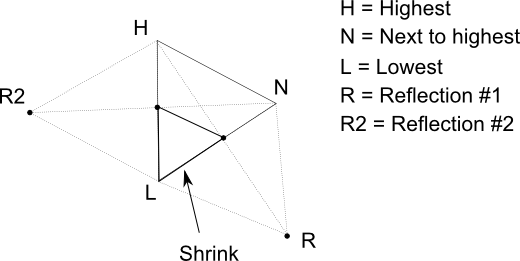
\includegraphics[width=10cm]{spendley-steps.png}
\end{center}
\caption{Spendley et al. simplex moves}
\label{fig-spendley-moves}
\end{figure}

The various situations in which these moves are chosen are 
presented in figures \ref{fig-spendley-moves-reflect}, \ref{fig-spendley-moves-reflect2}
and \ref{fig-spendley-moves-shrink}.

The basic move is the reflection step, presented in figure 
\ref{fig-spendley-moves-reflect} and \ref{fig-spendley-moves-reflect2}. 
These two figures shows that the Spendley et al.
algorithm is based on a discretization of the parameter space. 
The optimum is searched on that grid, which is based on regular simplices.
When no move is possible to improve the situation on that grid,
a shrink step is necessary, as presented in figure \ref{fig-spendley-moves-shrink}.

\begin{figure}
\begin{center}
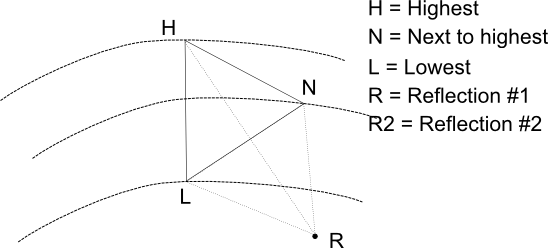
\includegraphics[width=10cm]{spendley-steps-reflect.png}
\end{center}
\caption{Spendley et al. simplex moves - reflection with respect to highest point}
\label{fig-spendley-moves-reflect}
\end{figure}

\begin{figure}
\begin{center}
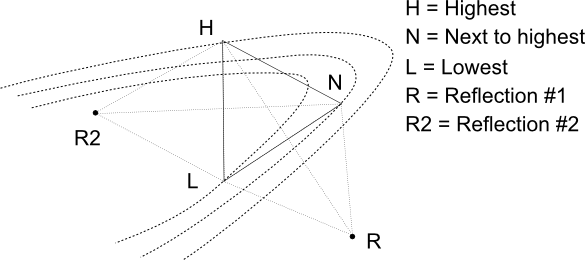
\includegraphics[width=10cm]{spendley-steps-reflect2.png}
\end{center}
\caption{Spendley et al. simplex moves - reflection with respect to next-to-highest point. 
It may happen that the next iteration is a shrink step.}
\label{fig-spendley-moves-reflect2}
\end{figure}

In the situation of figure \ref{fig-spendley-moves-shrink}, neither the 
reflection \#1 or reflection \#2 have improved the simplex. 
Diminishing the size of the simplex by performing a shrink step 
is the only possible move because the 
simplex has vertices which are located across the valley.
This allows to refine the discretization grid on which the 
optimum is searched.

\begin{figure}
\begin{center}
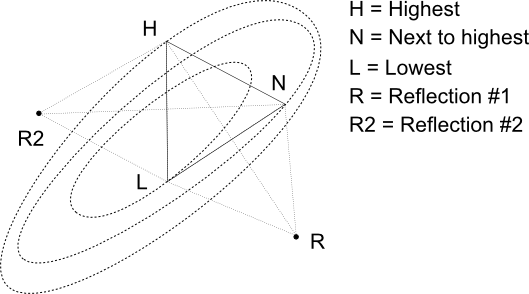
\includegraphics[width=10cm]{spendley-steps-shrink.png}
\end{center}
\caption{Spendley et al. simplex moves - shrink.}
\label{fig-spendley-moves-shrink}
\end{figure}

\subsection{Termination criteria}

TODO...

\section{Numerical experiments}

In this section, we present some numerical experiments 
with the Spendley et al. algorithm.

\subsection{Quadratic function}

The function we try to minimize is the following quadratic 
in 2 dimensions 

\begin{eqnarray}
f(x_1,x_2) = x_1^2 + x_2^2 - x_1 x_2
\end{eqnarray}

The stopping criteria is based on the relative size of the simplex 
with respect to the size of the initial simplex 

\begin{eqnarray}
\sigma(S) < tol \times \sigma(S_0)
\end{eqnarray}

The initial simplex is a regular simplex with length unity.
The numerical results are presented in table \ref{fig-spendley-numexp1-table}.

\begin{figure}[htbp]
\begin{center}
\begin{tiny}
\begin{tabular}{|l|l|}
\hline
Iterations & 49 \\
Function Evaluations & 132 \\
$x_0$ & $(2.0,2.0)$ \\
Relative tolerance on simplex size & $10^{-8}$ \\
Exact $x^\star$ & $(0.,0.)$\\
Computed $x^\star$ & $(2.169e-10, 2.169e-10)$\\
Computed $f(x^\star)$ & $4.706e-20$\\
\hline
\end{tabular}
\end{tiny}
\end{center}
\caption{Numerical experiment with Spendley's et al. method on the quadratic function
$f(x_1,x_2) = x_1^2 + x_2^2 - x_1 x_2$}
\label{fig-spendley-numexp1-table}
\end{figure}


The various simplices generated during the iterations are 
presented in figure \ref{fig-spendley-numexp1-historysimplex}.
The method use reflections in the early iterations. Then there
is no possible improvement using reflections and shrinking is necessary.
That behaviour is an illustration of the discretization which has already
been discussed.

\begin{figure}
\begin{center}
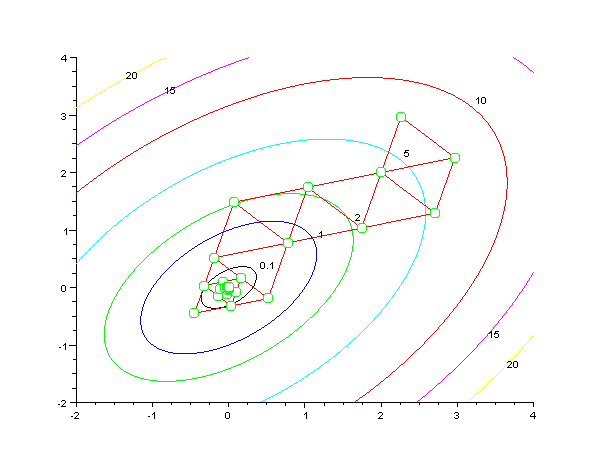
\includegraphics[width=10cm]{quad2bis-spendley-simplexcontours.png}
\end{center}
\caption{Spendley et al. numerical experiment -- history of simplex}
\label{fig-spendley-numexp1-historysimplex}
\end{figure}

The figure \ref{fig-spendley-numexp1-sigma} presents the history of the oriented
length of the simplex. The length is updated step by step, where each step 
corresponds to a shrink in the algorithm.

\begin{figure}
\begin{center}
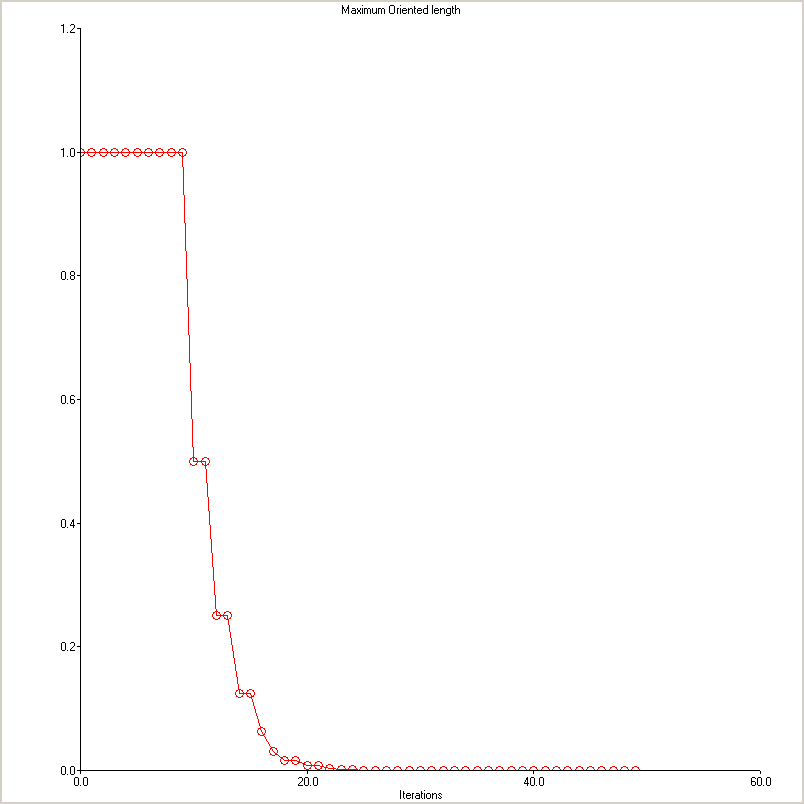
\includegraphics[width=10cm]{quad2bis-spendley-history-sigma.png}
\end{center}
\caption{Spendley et al. numerical experiment -- history of length of simplex}
\label{fig-spendley-numexp1-sigma}
\end{figure}

The convergence is quite fast in this case, since less than 60 iterations
allow to get a function value lower than $10^{-15}$, as shown in 
figure \ref{fig-spendley-numexp1-logfopt}.

\begin{figure}
\begin{center}
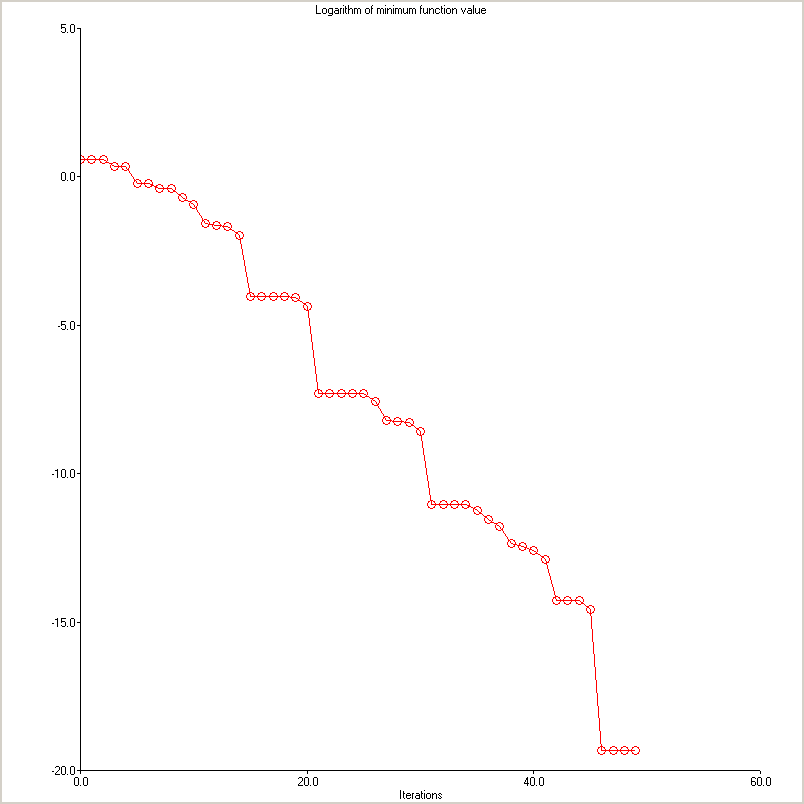
\includegraphics[width=10cm]{quad2bis-spendley-history-logfopt.png}
\end{center}
\caption{Spendley et al. numerical experiment -- history of logarithm of function}
\label{fig-spendley-numexp1-logfopt}
\end{figure}

\subsection{Badly scaled quadratic function}

The function we try to minimize is the following quadratic 
in 2 dimensions 
\begin{eqnarray}
\label{quadratic-sp-function2}
f(x_1,x_2) = a x_1^2 + x_2^2,
\end{eqnarray}
where $a>0$ is a chosen scaling parameter. 
The more $a$ is large, the more difficult the problem is 
to solve with the simplex algorithm.

We set the maximum number of function evaluations to 400.
The initial simplex is a regular simplex with length unity.

The numerical results are presented in table \ref{fig-spendley-numexp1-table},
where the experiment is presented for $a=100$. One can check that the 
number of function evaluation is equal to its maximum limit, even if the value of the 
function at optimum is very inacurate ($f(x^\star) \approx 0.08$).

\begin{figure}[h]
\begin{center}
\begin{tiny}
\begin{tabular}{|l|l|}
\hline
Iterations & 340 \\
Function Evaluations & 400 \\
$a$ & $100.0$ \\
$x_0$ & $(10.0,10.0)$ \\
Relative tolerance on simplex size & $10^{-8}$ \\
Exact $x^\star$ & $(0.,0.)$\\
Computed $x^\star$ & $(0.001,0.2)$\\
Computed $f(x^\star)$ & $0.08$\\
\hline
\end{tabular}
\end{tiny}
\end{center}
\caption{Numerical experiment with Spendley's et al. method on a badly scaled quadratic function}
\label{fig-spendley-numexp2-table}
\end{figure}


The various simplices generated during the iterations are 
presented in figure \ref{fig-spendley-numexp2-historysimplex}.
The method use reflections in the early iterations. Then there
is no possible improvment using reflections and shrinking is necessary.
But the shrinking makes the simplex very small so that a large number of 
iterations are necessary to improve the function value.
This is a limitation of the method, which is based on a simplex 
which can vary its size, but not its shape.

\begin{figure}
\begin{center}
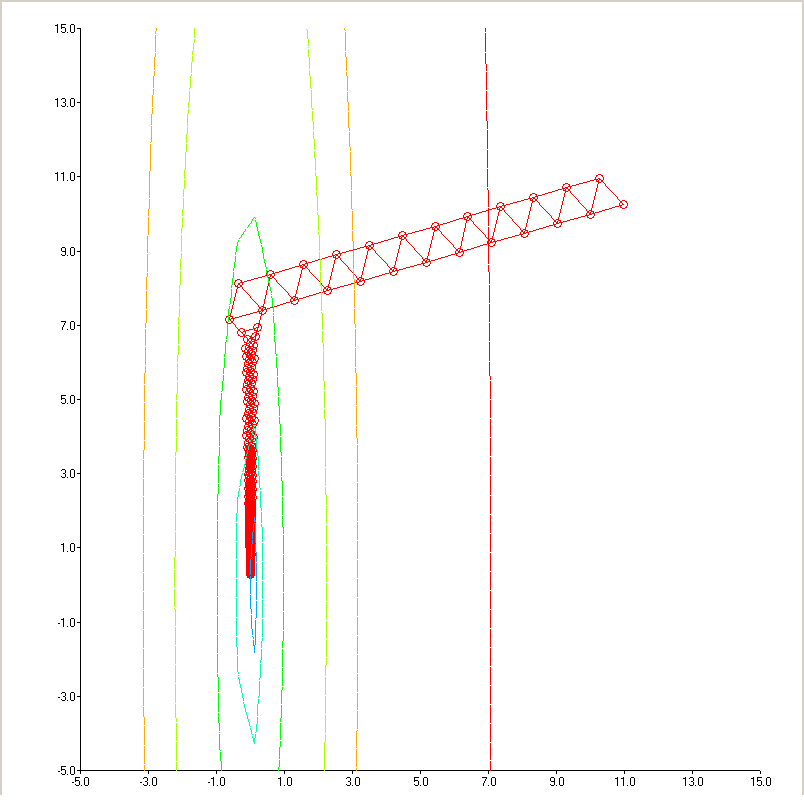
\includegraphics[width=10cm]{quad2-spendley-simplexcontours.png}
\end{center}
\caption{Spendley et al. numerical experiment with $f(x_1,x_2) = (a * x_1)^2 + x_2^2$ and $a=100$ -- history of simplex}
\label{fig-spendley-numexp2-historysimplex}
\end{figure}

In figure \ref{fig-spendley-numexp2-scaling}, we analyse the 
behaviour of the method with respect to scaling.
We check that the method behave poorly when the scaling is 
bad. The convergence speed is slower and slower and impractical 
when $a>10$

\begin{figure}[htbp]
\begin{center}
\begin{tiny}
\begin{tabular}{|l|l|l|}
\hline
$a$ & Function evaluations & Computed $f(x^\star)$ \\
$1.0$ & 160 & $2.35e-18$ \\
$10.0$ & 222 & $1.2e-17$ \\
$100.0$ & 400 & $0.083$ \\
$1000.0$ & 400 & $30.3$ \\
$10000.0$ & 400 & $56.08$ \\
\hline
\end{tabular}
\end{tiny}
\end{center}
\caption{Numerical experiment with Spendley's et al. method on a badly scaled quadratic function}
\label{fig-spendley-numexp2-scaling}
\end{figure}

\subsection{Sensitivity to dimension}

In this section, we try to study the convergence of the 
Spendley et al. algorithm with respect to the number of variables.
The function we try to minimize is the following quadratic 
in n-dimensions 
\begin{eqnarray}
\label{quadratic-sp-function3}
f(x_1,x_2) = \sum_{i=1,n} x_i^2.
\end{eqnarray}

The initial simplex is a regular simplex with length unity.
The initial guess is at 0 so that this vertex is never updated 
during the iterations.

For this test, we compute the rate of convergence as presented
in Han \& Neuman. This rate is defined as 

\begin{eqnarray}
\label{rho-sp-rate-convergence}
\rho(S_0,n) = \textrm{lim sup}_{k\rightarrow \infty} 
\left(\sum_{i=0,k-1} \frac{\sigma(S_{i+1}}{\sigma(S_i}\right)^{1/k}
\end{eqnarray}

That definition can be viewed as the geometric mean of the ratio of the 
oriented lengths between successive simplices and the minimizer 0.
This definition implies 

\begin{eqnarray}
\label{rho-sp-rate-convergence2}
\rho(S_0,n) = \textrm{lim sup}_{k\rightarrow \infty} 
\left( \frac{\sigma(S_{k+1}}{\sigma(S_0}\right)^{1/k}
\end{eqnarray}

The figure \ref{fig-sp-numexp3-dimension} presents the results of this 
experiment for $n=1,20$. 

The number and kids of performed steps are presented in figure \ref{fig-sp-numexp3-nbsteps}.
It must be noticed that reflection step occurs rarely during the iterations : the algorithm mostly performs 
shrink steps.

\begin{figure}[htbp]
\begin{center}
\begin{tiny}
\begin{tabular}{|l|l|l|l|}
\hline
$n$ & \# Reflections & \# Reflection & \#Shrink\\
 & / High & / Next to High & \\
\hline
1 & 0 & 0 & 27\\
2 & 0 & 0 & 27\\
3 & 1 & 0 & 27\\
4 & 5 & 1 & 27\\
5 & 0 & 0 & 27\\
6 & 6 & 0 & 27\\
7 & 4 & 0 & 27\\
8 & 0 & 0 & 27\\
9 & 12 & 1 & 27\\
10 & 0 & 0 & 27\\
11 & 0 & 0 & 27\\
12 & 14 & 0 & 27\\
13 & 0 & 0 & 27\\
14 & 24 & 3 & 27\\
15 & 0 & 0 & 27\\
16 & 0 & 0 & 27\\
17 & 21 & 0 & 27\\
18 & 0 & 0 & 27\\
19 & 28 & 0 & 27\\
\hline
\end{tabular}
\end{tiny}
\end{center}
\caption{Numerical experiment with Spendley et al method on a generalized quadratic function -- number 
and kinds of steps performed}
\label{fig-sp-numexp3-nbsteps}
\end{figure}

One can check that the number of function evaluations 
increases approximately linearily with the dimension of the problem in
figure \ref{fig-sp-numexp3-fvn}. A rough rule of thumb is that, for $n=1,19$, 
the number of function evaluations is equal to $30n$.
This test is in fact the best that we can expect from this algorithm : since 
most iterations are shrink steps, most iterations improves the function value.

\begin{figure}[htbp]
\begin{center}
\begin{tiny}
\begin{tabular}{|l|l|l|l|}
\hline
$n$ & Function evaluations & Iterations & $\rho(S_0,n)$\\
\hline
1 & 83 & 28 & 0.5125321059829373\\
2 & 111 & 28 & 0.5125321059829373\\
3 & 140 & 29 & 0.52448212766151725\\
4 & 174 & 34 & 0.57669577295965202\\
5 & 195 & 28 & 0.5125321059829373\\
6 & 229 & 34 & 0.57669577295965202\\
7 & 255 & 32 & 0.55719337129794622\\
8 & 279 & 28 & 0.5125321059829373\\
9 & 321 & 41 & 0.63352059021162177\\
10 & 335 & 28 & 0.5125321059829373\\
11 & 363 & 28 & 0.5125321059829373\\
12 & 405 & 42 & 0.64044334488213628\\
13 & 419 & 28 & 0.5125321059829373\\
14 & 477 & 55 & 0.71157656804932146\\
15 & 475 & 28 & 0.5125321059829373\\
16 & 503 & 28 & 0.5125321059829373\\
17 & 552 & 49 & 0.68253720379799854\\
18 & 559 & 28 & 0.5125321059829373\\
19 & 615 & 56 & 0.71591347660379834\\
\hline
\end{tabular}
\end{tiny}
\end{center}
\caption{Numerical experiment with Spendley et al. method on a generalized quadratic function}
\label{fig-sp-numexp3-dimension}
\end{figure}

\begin{figure}
\begin{center}
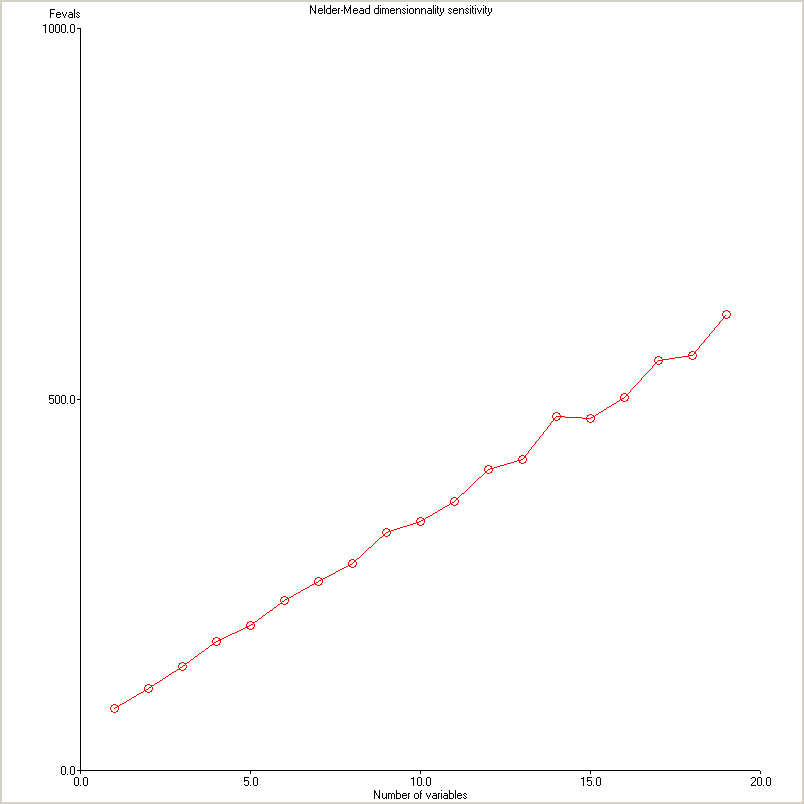
\includegraphics[width=10cm]{spendley-dimension-nfevals.png}
\end{center}
\caption{Spendley et al. numerical experiment -- number of function evaluations 
depending on the number of variables}
\label{fig-sp-numexp3-fvn}
\end{figure}

The figure \ref{fig-nm-numexp3-rho} presents the rate of convergence 
depending on the number of variables. The figure shows that 
the rate of convergence rapidly gets close to 1 when the number 
of variables increases. That shows that the rate of convergence 
is slower and slower as the number of variables increases, as 
explained by Han \& Neuman.

\begin{figure}
\begin{center}
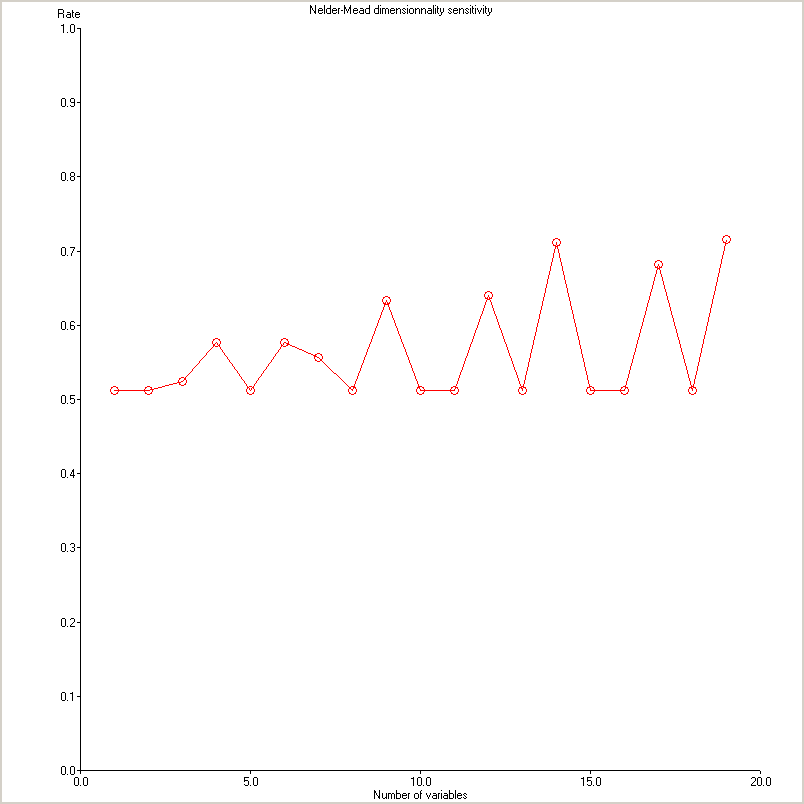
\includegraphics[width=10cm]{spendley-dimension-rho.png}
\end{center}
\caption{Spendley et al. numerical experiment -- rate of convergence 
depending on the number of variables}
\label{fig-sp-numexp3-rho}
\end{figure}

\section{Conclusion}

We saw in the first numerical experiment that the method 
behave reasonably when the function is correctly scaled.
When the function is badly scaled, as in the second numerical 
experiment, the Spendley et al. algorithm produces a large 
number of function evaluations and converges very slowly.
This limitation occurs with even moderate badly scaled 
functions and generates a very slow method in these 
cases.


